\documentclass{beamer}
\DeclareGraphicsExtensions{.pdf,.png,.jpg,.eps}
\setbeamertemplate{caption}{\raggedright\insertcaption\par}
\title{Savings, Savings, Savings}
\author{Gabriel C-Parent}
\date{IFT6751 H2015}


\usetheme{Execushares}

\begin{document}
\maketitle

\begin{frame}
\frametitle{Overview}
\begin{itemize}
	\item cvrp problem
	\item implementation details
	\item improvement procedures
	\item construction procedure
	\item genetic algorithm
	\item tabu search
	\item QA
\end{itemize}
\end{frame}


\section{The Problem}

\begin{frame}
\frametitle{Capacitated Vehicle Routing}
\begin{center}

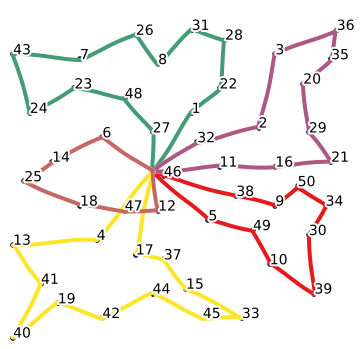
\includegraphics[scale=0.25]{figs/cvrp}


\begin{equation*}
\begin{aligned}
& \text{minimize}
& & \sum\limits_{route \in solution} distance(route) \\
& \text{subject to}
& & weight(route) \leq vehicle\ capacity
\end{aligned}
\end{equation*}

\end{center}
\end{frame}


\section{Implementation}

\begin{frame}
\frametitle{Implementation Details}
\begin{center}

\includegraphics[scale=0.4]{figs/tools}

\end{center}
\end{frame}


\begin{frame}
\frametitle{Implementation Details}
\begin{itemize}
	\item reuse basic operators
	\item modularity
	\item concise
\end{itemize}
\end{frame}

\section{Improvement}
\subsection{2-opt descent (TSP)}

\begin{frame}
\frametitle{2-opt descent}
\begin{itemize}
	\item uses common 2-opt operator
	\item calculates all possible 2-opt for each iteration
	\item chooses the best available
\end{itemize}
\end{frame}

\begin{frame}
\frametitle{2-opt example}
\begin{center}
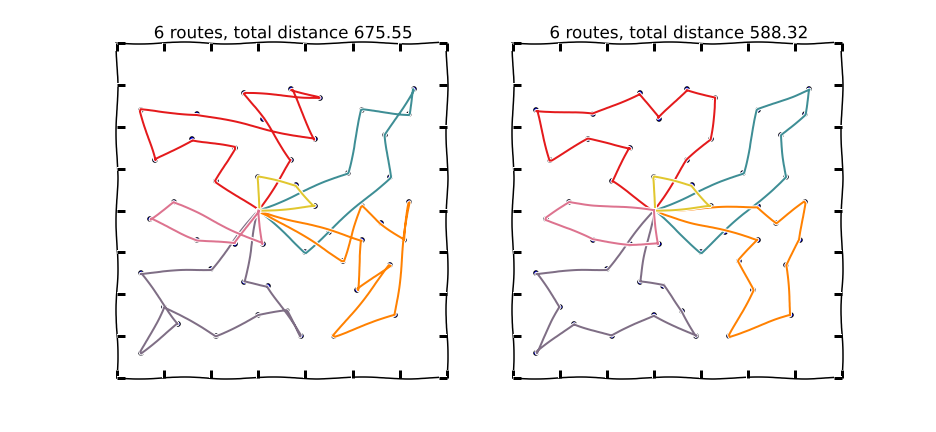
\includegraphics[scale=0.3]{figs/2opt}

\end{center}
\end{frame}


\subsection{$\lambda_1$-interchange descent}

\begin{frame}
\frametitle{$\lambda_1$-interchange definition}
\begin{itemize}
	\item $\lambda$-interchange, Osman, 1991
	\item exchange of customers between routes
	\item only feasible exchanges (capacity constraint)
	\item insertion (1, 0) and (0, 1) or interchange (1, 1)
	\item chooses the best option at each iteration
	\item apply 2-opt descent on routes implicated
\end{itemize}
\end{frame}


\begin{frame}
\frametitle{$\lambda_1$-interchange example}
\begin{center}
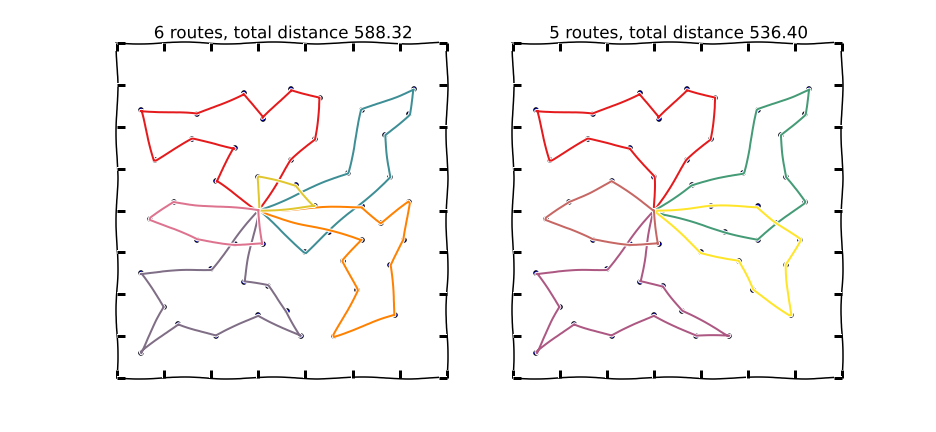
\includegraphics[scale=0.3]{figs/lambda}

\end{center}
\end{frame}

\section{Construction}


\subsection{Random Savings}

\subsection{General Concepts}
\begin{frame}
\frametitle{Random Savings Definition}
\begin{itemize}
	\item iterated local search
	\item variant of parallel savings
	\item at each iteration select randomly from top $k$ best savings
	\item $k$=1 $\rightarrow$ normal parallel savings
	\item once finished, apply improvement method
		
\end{itemize}
\end{frame}


\subsection{Results}
\begin{frame}
\frametitle{Random Savings, k=5}
\begin{center}
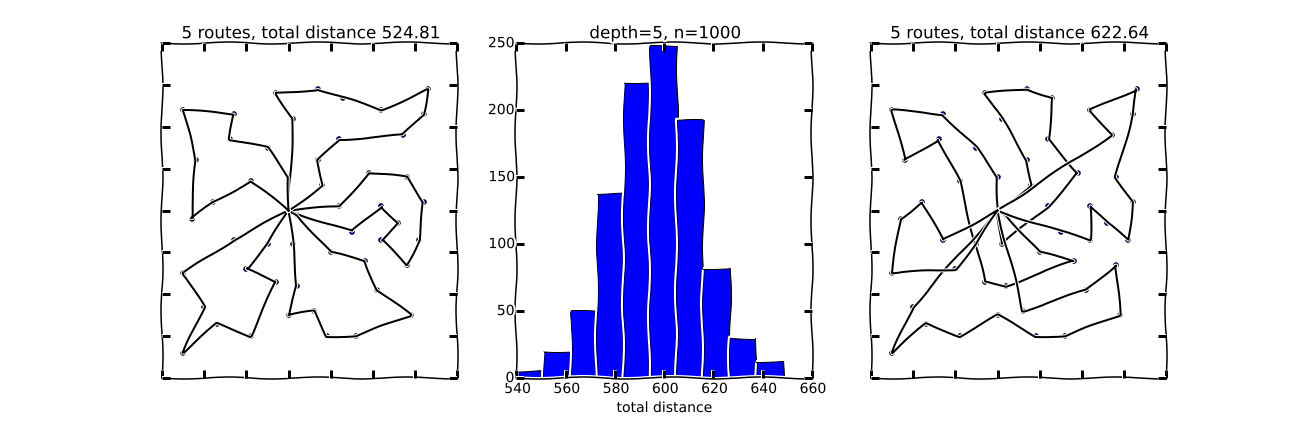
\includegraphics[scale=0.25]{figs/random_savings5}

\end{center}
\end{frame}


\begin{frame}
\frametitle{Random Savings, k=10}
\begin{center}
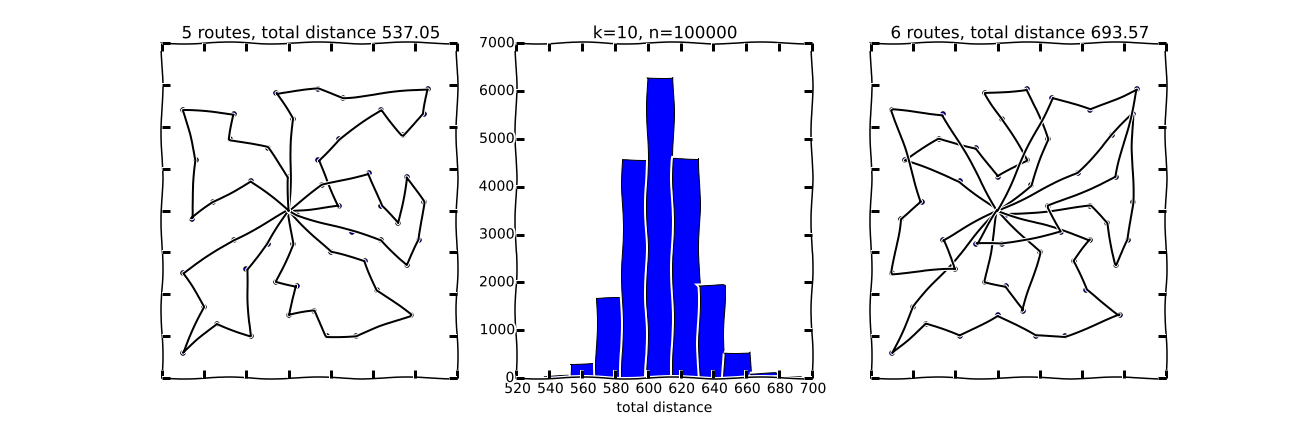
\includegraphics[scale=0.25]{figs/random_savings10}

\end{center}
\end{frame}


\begin{frame}
\frametitle{Best result in 60 secs}
\begin{center}
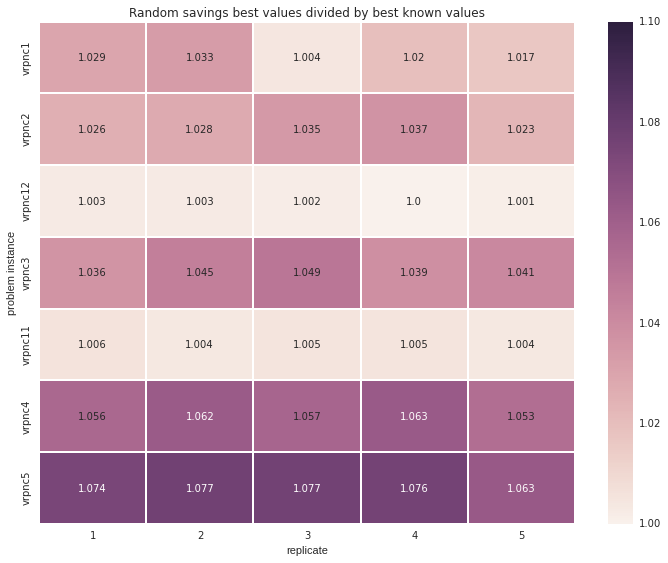
\includegraphics[scale=0.25]{figs/rs_best}

\end{center}
\end{frame}



\section{Genetic Algorithm}




\subsection{Crossover}

\begin{frame}
\frametitle{Crossover Description}

\begin{itemize}
	\item[1] arrange routes by angle of centroid to depot
	\item[2] choose $\frac{n}{4}$ contiguous routes from parent 1
	\item[3] choose at most $\frac{n}{4}$ contiguous non-intersecting routes from parent 2
	\item[4] assign routes to the rest of clients using parallel savings 
\end{itemize}

\end{frame}



\begin{frame}
\frametitle{Crossover example}
\begin{center}
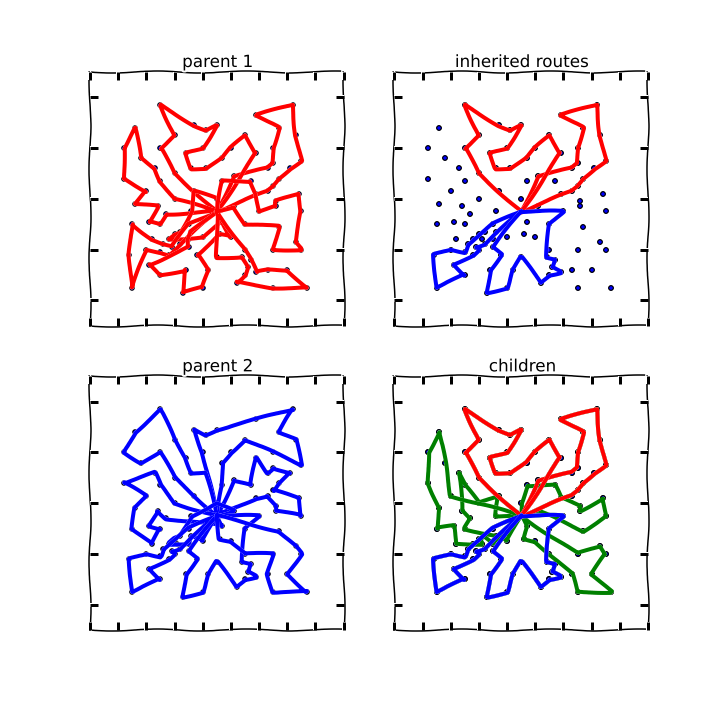
\includegraphics[scale=0.25]{figs/crossover}

\end{center}

\begin{center}
\end{center}
\end{frame}




\subsection{Mutation}
\begin{frame}
\frametitle{Mutation Description}
\begin{itemize}
	\item reuse the $\lambda_1$-interchange operator
	\item use a fixed (in this case 5) number of iterations
	\item serves as local exploration and changes clusters of clients
\end{itemize}
\end{frame}


\begin{frame}
\frametitle{Mutation example}
\begin{center}
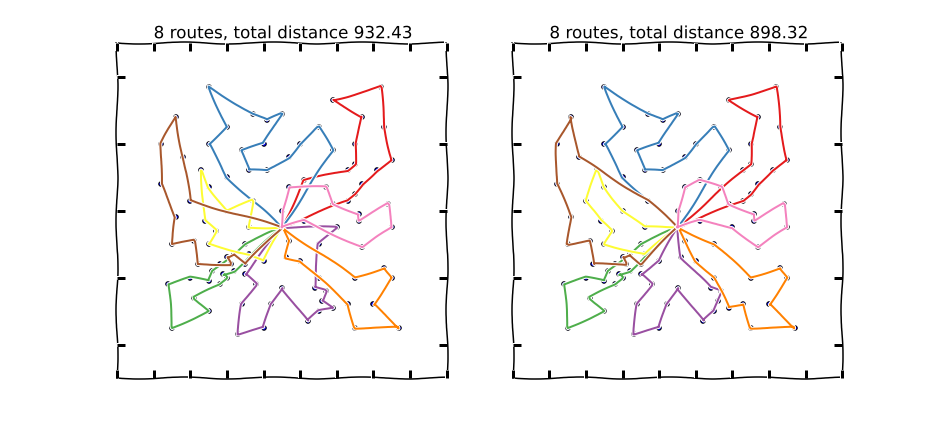
\includegraphics[scale=0.3]{figs/mutation}
\end{center}

\end{frame}


\subsection{Free Parameters}
\begin{frame}
\frametitle{Genetic Algorithm Parameters}
\begin{center}
\begin{itemize}
	\item number of generations
	\item population size
	\item elitism (percentage of transfer)
	\item recombination probability
	\item mutation probability
	\item $k$ for random savings
\end{itemize}

\end{center}
\end{frame}

\subsection{Results}
\begin{frame}
\frametitle{Results}
\begin{center}
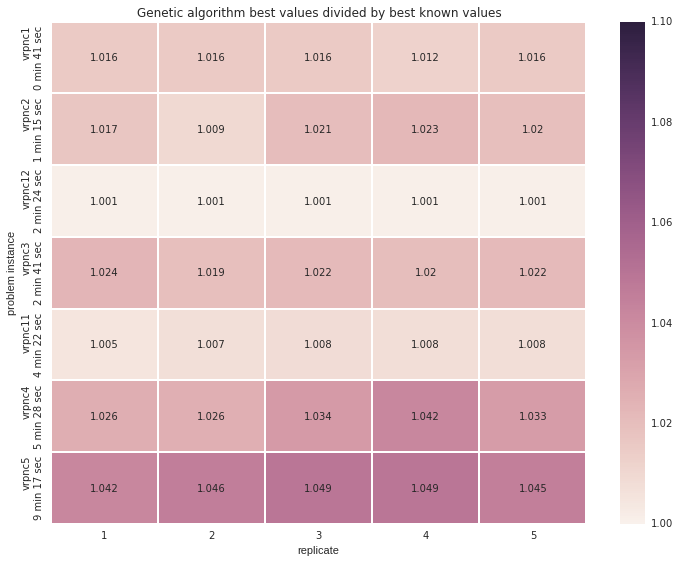
\includegraphics[scale=0.25]{figs/ga_best}

\end{center}
\end{frame}

\section{Tabu Search}

\subsection{Tabu Search Description}

\begin{frame}
\frametitle{Tabu Search Description}
\begin{itemize}
	\item Neighbourhood Structure
	\item Tabu List
	\item Diversification
\end{itemize}
\end{frame}


\subsection{Neighbourhood Structure}

\begin{frame}
\frametitle{Neighbourhood Structure}
\begin{itemize}
	\item $\lambda_1$-interchange
	\item only feasible solutions
\end{itemize}
\end{frame}


\subsection{Tabu List}

\begin{frame}
\frametitle{Tabu List}
\begin{itemize}
	\item avoid reversing a move
	\item remember pairs $(client,\ route)$
	\item $max\{7,\ -40 + 9.6 \times ln(n \times v)\}$
\end{itemize}
\end{frame}


\subsection{Diversification}

\begin{frame}
\frametitle{Diversification by Multi-Start}
\begin{itemize}
	\item takes a parameter called $patience$
	\item patience replenish after a new best is found
	\item patience runs out $\rightarrow$ random savings
\end{itemize}
\end{frame}

\subsection{Results}

\begin{frame}
\frametitle{Best Results in 60 sec}
\begin{center}
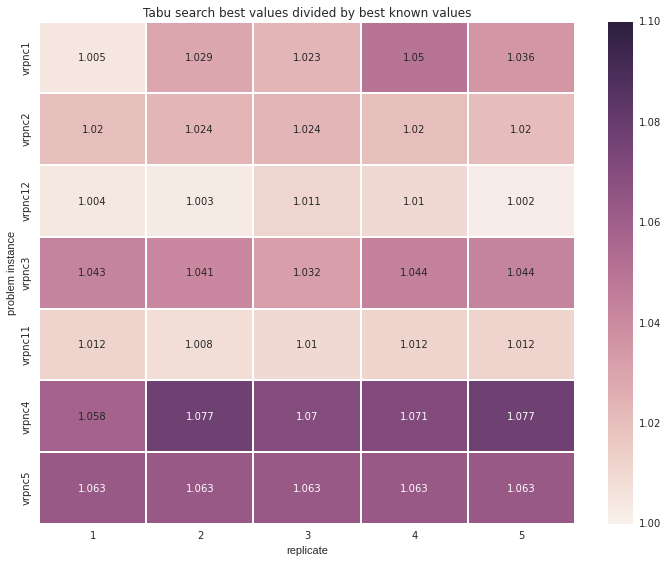
\includegraphics[scale=0.25]{figs/tabu_search}

\end{center}
\end{frame}



\section{Overall Performance}

\begin{frame}
\frametitle{Overall Performance}
\begin{itemize}
	\item complexity : [RS, GA, Tabu]
	\item speed: [Tabu, RS, GA]
	\item quality: [GA/Tabu, RS]
\end{itemize}
\end{frame}


\section{QA}


\end{document}